\documentclass[12pt]{ruthesis}
\usepackage{amsmath}
\usepackage{amssymb}
\usepackage{latexsym}
\usepackage{graphics}
\usepackage{epsfig,epsf,rotating}
\usepackage{graphicx}
\usepackage{subcaption}
%\usepackage{pictex}
\usepackage{epsf}
\usepackage{svg}
%\usepackage{cite}
\usepackage{theorem}
\newtheorem{proposition}{Proposition}

\theoremheaderfont{\itshape} {\theoremstyle{break}
\newtheorem{Fact}{Fact}[chapter]} \theoremstyle{break}
\newtheorem{Lem}{Lemma}[chapter] \theoremstyle{break}
\newtheorem{Thm}{Theorem}[chapter] {\theoremstyle{plain}
  \theorembodyfont{\rmfamily}  \newtheorem{Prf}{Proof}[chapter]}
{\theoremstyle{plain}
  \theorembodyfont{\rmfamily}  \newtheorem{Def}{Definition}[chapter]}

\title{Ultrafast Spectroscopy of (6,5) Carbon Nanotubes}
\ctitle{Sphere detection and LDPC decoding algorithms and architectures for wireless systems}
\author{Bryan E. Anthonio}
\department{Applied Physics}
\school{Rice University}
\degree{Master of Science}

\committee {
        Junichiro Kono, Chair \\
        Professor of Electrical \& Computer Engineering, Physics \& Astronomy,
        Materials Science \& NanoEngineering \and
        Hanyu Zhu \\
        Assistant Professor of Materials Science \& NanoEngineering \and
        Bruce Weisman \\
        Associate Professor of Chemistry, Materials Science \& NanoEngineering \and
}

\address{Houston, Texas}
\donemonth{October} \doneyear{2019} \makeindex
\begin{document}

  \begin{frontmatter}
   \pagenumbering{roman}
   %\makecover
   \maketitle
   \thispagestyle{empty}
\begin{abstract}
Single-wall carbon nanotubes (SWCNTs) represent an exemplary model system for studying one-dimensional (1-D) physics in condensed matter research. Conceptually, they can be presented as a rolled-up sheet of graphene, and depending on their crystal structure they either exhibit properties of semiconductors or metals. These materials also feature strong Coulomb interactions that have profound effects, giving rise to optical properties which differ from those of 2-D and 3-D materials. Chief amongst these properties is the tendency for optical excitations to only generate bound electron-hole pairs in SWCNTs, known as excitons, rather than free electron-hole pairs. In this thesis, we used ultrafast optical pump-probe spectroscopy to investigate both coherent and noncoherent phenomena in (6,5) SWCNTs. The samples used for this investigation included two different ensembles of individually-suspended (6,5)-enriched SWCNTs in solution. In one ensemble, the SWCNTs were suspended in an aqueous solution containing surfactants, whereas the SWCNTs in the other ensemble were suspended using an aromatic polymer in a toluene solution. In this study, we observed a coherent blueshift of the lowest-lying exciton resonance when the SWCNTs were photoexcited below the band gap, a signature of the optical Stark effect. When photoexciting the samples at the second-highest exciton resonance, we observed quenching of the lowest exciton resonance for the SWCNTs in the aqueous suspension but not for those that were suspended in toluene. This observation alone raises further questions regarding how the dielectric environment surrounding
 SWCNTs affects the carrier dynamics that they exhibit.
\end{abstract}

   %\include{ack}
   \tableofcontents
   \listoffigures
   \listoftables
%   \include{ded}
  \end{frontmatter}
\pagenumbering{arabic}

\linespacing{1.7}

\chapter{Introduction}

Carbon nanotubes interesting. 2D sheets of graphene rolled into cylindrical structure. Allow us to explore physics of 1-D materials. 

\begin{figure}[H]
	\centering
	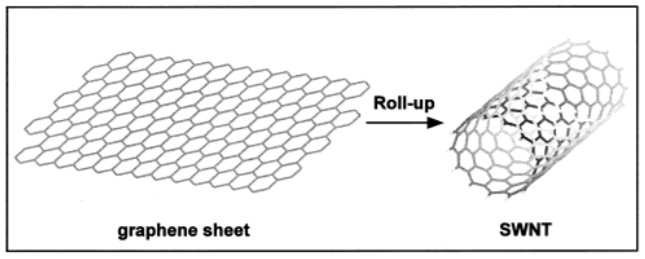
\includegraphics{images/chapter_intro/rolled_up_graphene.png}
	\caption{Carbon nanotubes can be conceptualized as a graphene sheet that has been rolled up to form a cylindrical structure. Reproduced from \cite{odom2000structure}.}
\end{figure}

Applications in electronic and optoelectronic devices such as transistors, detectors, polarizers, etc. 

The purpose of this thesis focuses on elucidating the ultrafast dynamics of single-wall carbon nanotubes. Ultrafast spectroscopy incorporates the use of laser pulses to characterize the dynamics of microscopic phenomena occuring in many different materials \cite{shah1996ultrafast}. Probe interrogates sample properties. Adjusting the arrival time delay between pump and probe makes it possible to measure dynamics of sample properties with femtosecond resolution.

Previous studies used samples with several different chirlaties, making it harder to distinguish between the dynamics of each chirality. Recent developments have make it possible to make high-purity, single-chirality samples. 

Chapter 2 provides an introduction to the some of the basic properties of carbon nanotubes. Chapter 3 explores prior works ultrafast spectroscopy measurements of carbon nanotubes. Chapter 4 illustrates the relevant experimental procedures. Chapter 5 presents coherent processes that have been observed. Chapter 6 discusses dynamics that occur after pumping above the bandgap.
\chapter{Experimental Procedures}

\section{(6,5) Carbon Nanotube Sample Properties}

\subsection{Sample Preparation}
The sample preparation procedure is well described by Ref \cite{ichinose2017extraction}. For preparing a high-purity (6,5) sample, the process starts with obtaining a CoMoCat solution (Sigma-Aldrich) containing several different chiralities of carbon nanotubes. Gel chromatography is then performed on this mixture to isolate a solution containing a high concentration of (6,5) nanotubes. In this process, the presence of a small concentration (4\%) of sodium deoxycholate (DOC), a surfactant, in the solution prevents nanotubes from clumping together to form bundles. Finally, the sample is pipetted into a quartz cuvette with an optical path length of 1 mm. 

%Include figure of absorption spectrum
\subsection{Sample Absorbance Spectrum}

Measuring the absorbance of prepared samples provides a means of determining the different chiralities present in the sample as well as their relative populations. Here, absorbance $A$ is defined as 

\begin{equation}
A = \log_{10}\left(\dfrac{I_{ref}}{I_{sample}}\right),
\end{equation}

where $I_{ref}$ and $I_{sample}$ represent the optical transmission through a reference sample and the nanotube sample respectively. The reference sample only contains water and a 4\% concentration of DOC and is also stored in a cuvette with an optical path length of 1 mm. 

Figure \ref{fig:sample_absorbance} presents the absorbance spectrum of the (6,5) sample measured using the white-light supercontinuum source described in section \ref{section:white_light_probe}. The spectrum exhibits a number of optical transitions including the $E_{11}$, phonon sideband, $E_{12}$, and $E_{22}$ resonances at photon energies of 1.26, 1.45, 1.9, and 2.17 eV respectively. Furthrmore, other small peaks in the sample at 1.35 and 1.41 eV emerge from exciton resonances of (9,1) and (6,4) nanotubes respectively.

\begin{figure}[H]
	\centering
	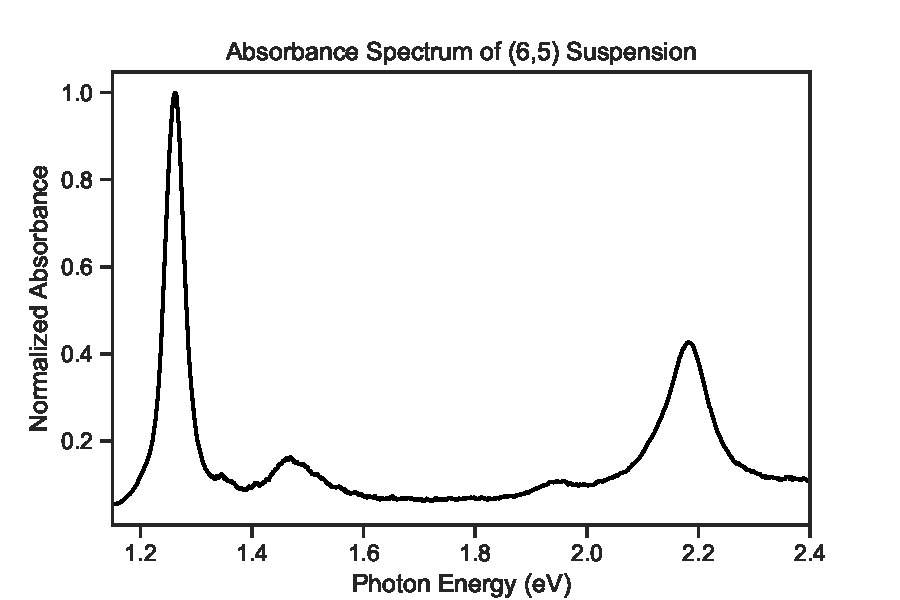
\includegraphics[scale=0.7]{images/chapter_methods/sample_absorbance}
	\caption{ Absorbance spectrum of (6,5) sample.}
	\label{fig:sample_absorbance}
\end{figure}

\section{Experimental Apparatus for Pump-Probe Spectroscopy}

%include figure of setup
\subsection{Overview}
The experimental apparatus, illustrated in Figure \ref{fig:setup_schematic}, incorporates the use of an intense optical pump pulse followed by a broadband probe pulse to characterize the ultrafast carrier dynamics of carbon nanotubes. The pump and probe beams are focused onto surface of the sample in a non-collinear geometry. Finally, the transmission spectrum of the probe is resolved using a spectrometer to resolve the non-equilibrium optical properties of the sample.  


\begin{figure}[h]
	\centering
	\includegraphics[scale=0.7]{example-image-a}
	\caption{ Schematic Diagram of the Experimental Apparatus. }
	\label{fig:setup_schematic}
\end{figure}


\subsection{Chirped Pulse Amplifier and Optical Parametric Amplifier}
The CPA-2010 laser source manufactured by Clark-MXR functions as the heart of this optical setup. This laser generates amplified pulses using a chirped pulse amplification process. It operates at a repetition rate of 1 KHz and outputs pulses with a 150 fs duration and a central wavelength of 775 nm. Finally, the CPA-2010 serves as a pump laser for the optical parametric amplifier (OPA). 

The OPA used in the setup is a TOPAS-800 produced by Light Conversion. It emits signal and idler beams via a superfluoresence in a barium borate (BBO) crystal which are then amplified in four subsequent stages. The signal and idler wavelengths span 1.1 - 1.5 $\mu$m  and 1.5 - 2.7 $\mu$m respectively. Furthermore, an additional BBO crystal placed at the output of the OPA provides a means of generating the second harmonic of the signal or idler which can be used an optical pump.

\subsection{Filters}

The setup features a wavelength separator that seperates the fundamental of the signal (FS) from the second harmonic of the signal (SHS). This optical device contains a set of two dichroic mirrors that reflect the SHS and transmit the FS. As a result of the second harmonic generation process, the polarization of SHS remains perpendicular to that of FS. Hence, a half-wave plate is placed in the optical path of the SHS and appropriately adjusted to make the polarizations of FS and SHS parallel to each other. 

In addition to this, two neutral density wheels are used to attenuate the intensity of the probe and the optical pump.

\subsection{White Light Continuum Probe}


\label{section:white_light_probe}
Supercontinuum generation represents a nonlinear optical process by which the spectrum of an incident laser pulse becomes significantly broadened \cite{dubietis2017ultrafast}. It has been observed to occur in many different media such as water, fused silica, sapphire and calcium fluoride \cite{dubietis2017ultrafast}. This process is facilitated by the formation of a filament which starts as a result of self-focusing \cite{dubietis2017ultrafast}. In other words, the refractive index of the supercontinuum generation medium depends on the intensity of propagating light \cite{dubietis2017ultrafast}. Due to the interplay between this self-focusing and other competing effects such as self-phase modulation, and multiphoton absorption, the spectrum  broadens as the pulse travels through the medium \cite{dubietis2017ultrafast}. 

In this setup, supercontinuum generation occurs by focusing the fundamental of the signal beam (FS) into a sapphire crystal with a thickness of 5 mm. Here, the center of the sapphire crystal is placed at a distance of one focal length of the lens used to focus the FS. This process generates a white-light continuum that spans 1 - 2.4 eV. 

Finally, an iris is placed in path of FS such that its aperture is positioned at the center of the FS beam. This iris is used to crop the outer portion of the FS, thereby reducing its the beam diameter. Doing this has been observed to have the effect of minimizing the temporal fluctuations of the generated white light spectrum. 

\subsection{Motorized Delay Stage and Optical Shutter}

The setup includes a motorized delay stage and an optical shutter that are used to control the pump conditions in each measurement.

The delay stage consists of a pair retro-reflecting mirrors mounted on a motorized stage. The pump beam travels to both of these mirrors. Hence, adjusting the position of the motorized stage alters the time delay between the pump and probe pulses by either increasing or decreasing the optical path length traveled by the pump pulse. 

The optical shutter makes it possible block the pump beam in order to measure probe transmission through the sample under equilibrium conditions. At each time delay, the transmission of the probe beam is measured with the pump beam blocked and with the pump beam unblocked by the shutter. Conducting measurements in this manner mitigates the effect of long-term fluctuations in the laser output. 

\subsection{Spectrometer}
The probe is collected into an optical fibre which sends the probe beam to a (\textbf{\color{red} NAME OF SPECTROMETER}) spectrometer built by Princeton Instruments.  The spectrometer uses a grating with a diffraction grating with a blaze wavelength of 800 nm and a groove density of (\textbf{\color{red} ADD GROOVE DENSITY}) per mm. The diffracted light is then imaged onto a CCD camera to measure the probe spectrum. 

The camera is silicon-based and contains an array of 1340 $\times$ 100 pixels. Finally, the camera must be cryogenically cooled to \SI{-100}{\celsius} using liquid nitrogen for an optimal signal-to-noise ratio.


\subsection{Pump and Probe Spot Sizes}
The pump and probe spot sizes are measured using a knife edge scan technique \cite{firester1977knife}. For this, a razor blade attached to a post is mounted on a motorized stage placed in the sample position. The sharp edge of the blade faces in a direction perpendicular to that of the direction of propagation of the incident beam. A power meter is placed behind the razor blade to measure the average power of the transmitted beams.

As the motorized stage moves the razor blade's position laterally with respect to the beam's propagation direction, the razor blade increasingly blocks portions of the incident beam.  Measuring the transmitted power of incident beam as a function of the razor blade position yields a cumulative distribution function of the incident light.

\begin{figure}[h]
	\centering
	\includegraphics[scale=0.7]{example-image-a}
	\caption{Example measurement of beam diameter for pump and probe. Solid lines are fits to the data using function defined in equation}
	\label{fig:beam_diamter_measurement}
\end{figure}

Assuming that the beam diameter can be approximated as a Gaussian distribution, the spot size can be estimated by fitting this data with the equation 

\begin{equation}
	P = P_0 + P_{max}/2 \left( 1 - \mathrm{erf} \left( \dfrac{\sqrt{2}(x - x_0)}{w} \right) \right),
\end{equation}

which represents the cumulative distribution function of a Gaussian distribution. This function yields the beam diameter $w$. Furthermore, $P_0$ represents the baseline of the power meter observed when the beam is fully blocked, erf stands for the standard error function, $P_{max}$ denotes the maximum power of the beam, $x$ parametrizes the position of the blade and $x_0$ indicates the position at which the blade blocks 50\% of the incident beam's average power.  








\chapter{Ultrafast Carrier Dynamics of (6,5) SWCNTs After Resonant E$_{22}$ Pumping}

\section{Overview}

This chapter presents an investigation of exciton-exciton annihilation in (6,5)-enriched suspensions using optical-pump, white-light probe measurements. The samples studied include one suspension of (6,5)-enriched SWCNTs dispersed using sodium deoxycholate (DOC) in an aqeuous solution and another and another set of polymer-wrapped (6,5)-enriched SWCNTs dispersed in toluene. All measurements were taken with optical pump photon energy equaling that of the $E_{22}$ resonance at 2.17 eV. Moreover, the measurements were conducted at room temperature under ambient conditions.

For the DOC-suspended sample, the aqueous solution slowly evaporated over time due to a crack in the quartz cuvette containing the dispersion. As a result, the concentration of SWCNTs steadily increased over time leading to an overall increase in optical absorption. This was accounted for by measuring the sample attenuance before each experiment to normalize the experimental data to ensure the consistency of the date. The PFO-wrapped sample was well sealed and no significant changes in the sample absorption were observed over time.


\section{Experimental Results}
Figures \ref{fig:weilu_cnt_time_traces} - \ref{fig:weilu_cnt_normalized_dt} present the data obtained from the DOC-suspended sample. Figure \ref{fig:weilu_cnt_time_traces} shows the normalized attenuance of the sample at indicated time delays using a pump power density of 7.82 GW/cm$^2$. Figure \ref{fig:weilu_cnt_max_decay} shows the maximum decay of the total attenuance within the spectral region of the $E_{11}$ resonance. Figure \ref{fig:weilu_cnt_max_decay_fit} shows the peak attenuance obtained in Figure \ref{fig:weilu_cnt_max_decay} as a function of the power density of the optical pump. Below power densities of 7.82 GW/cm$^2$, the peak attenuance decreases linearly with the power density. Figure \ref{fig:weilu_cnt_normalized_dt} shows the normalized differential transmission curves measured at the labeled power densities. The curves were fit using a bi-exponential decay model. Figure \ref{fig:weilu_cnt_decay_const} shows the fast and slow decay constants extracted from the fits shown in Figure \ref{fig:weilu_cnt_normalized_dt} (a).

Figure \ref{fig:jan_cnt_time_traces} shows the normalized attenuance of the sample at indicated time delays using a pump power density of 7.82 GW/cm$^2$. Figure \ref{fig:jan_cnt_max_decay} shows the maximum decay of the total attenuance within the spectral region of the $E_{11}$ resonance. Figure \ref{fig:jan_cnt_max_decay_fit} shows the peak attenuance obtained in Figure \ref{fig:jan_cnt_max_decay} as a function of the power density of the optical pump. Below power densities of 1.9 GW/cm$^2$, the peak attenuance decreases linearly with the power density. Figure \ref{fig:weilu_cnt_normalized_dt} shows the normalized differential transmission curves measured at the labeled power densities. The curves were fit using a bi-exponential decay model. Figure \ref{fig:weilu_cnt_decay_const} shows the fast and slow decay constants extracted from the fits shown in Figure \ref{fig:weilu_cnt_normalized_dt} (a).

\subsection{DOC-Suspended (6,5)-enriched Dispersion}



\begin{figure}[H]
	\centering
	{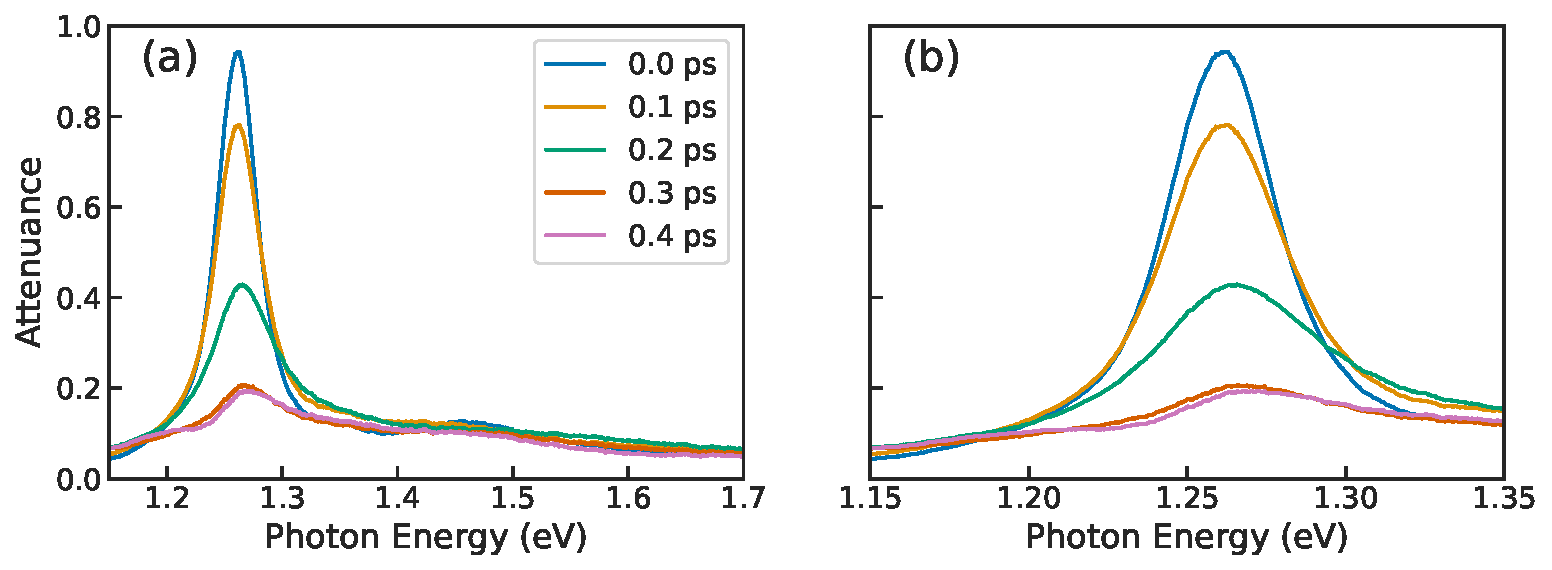
\includegraphics[height=2.4in]{images/chapter_my_data/Weilu_CNT_4mW_E11_decay} \phantomsubcaption}
	{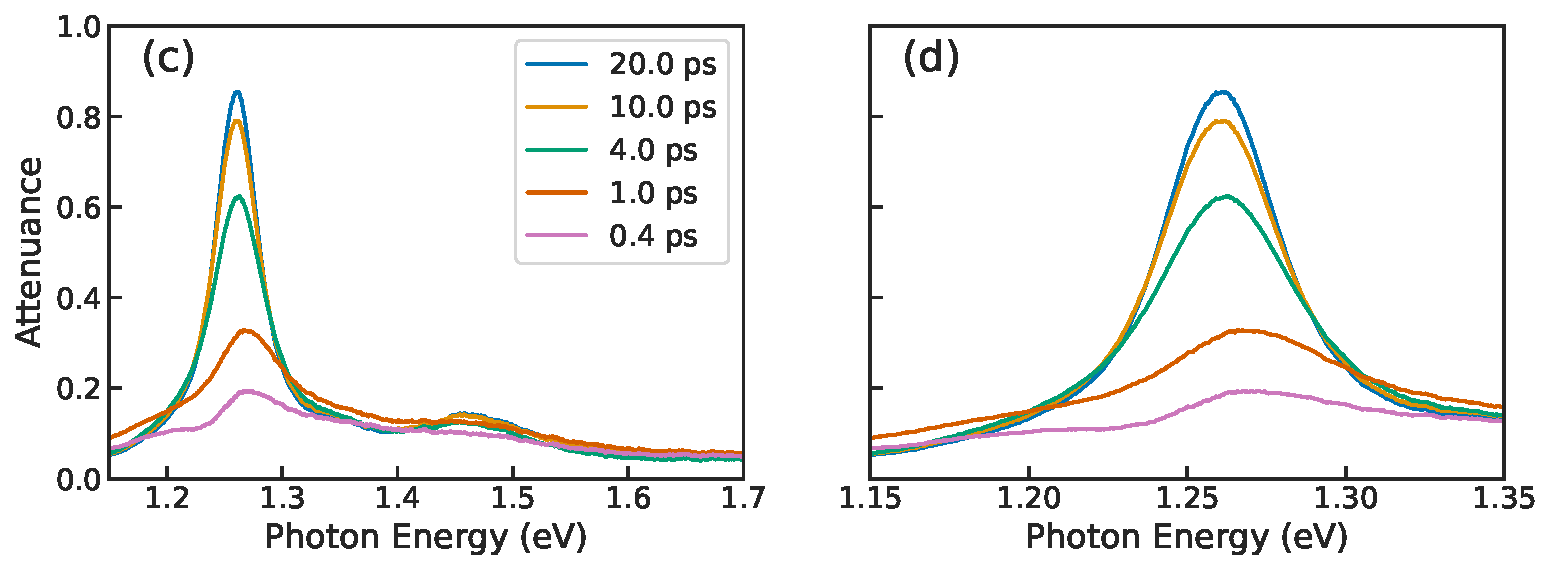
\includegraphics[height=2.4in]{images/chapter_my_data/Weilu_CNT_4mW_E11_recovery} \phantomsubcaption}
	\caption{Normalized attenuance traces measured at the indicated time delay after resonantly exciting the $E_{22}$ transition with a power density of 7.82 GW/cm$^2$. (a) Total attenuance showing the decay of the absorption at the $E_{11}$ peak at 1.26 eV as well as the attenuation of the phonon sideband located at 1.35 eV. (b) A close-up of the changes $E_{11}$ spectral region shown in Figure (a). (c) Total attenuance at later times showing the recovery of the $E_{11}$ and phonon sideband peaks. (d) A close-up of the changes $E_{11}$ spectral region shown in Figure (c).}
	\label{fig:weilu_cnt_time_traces}
\end{figure}

\begin{figure}[ht]
	\centering
	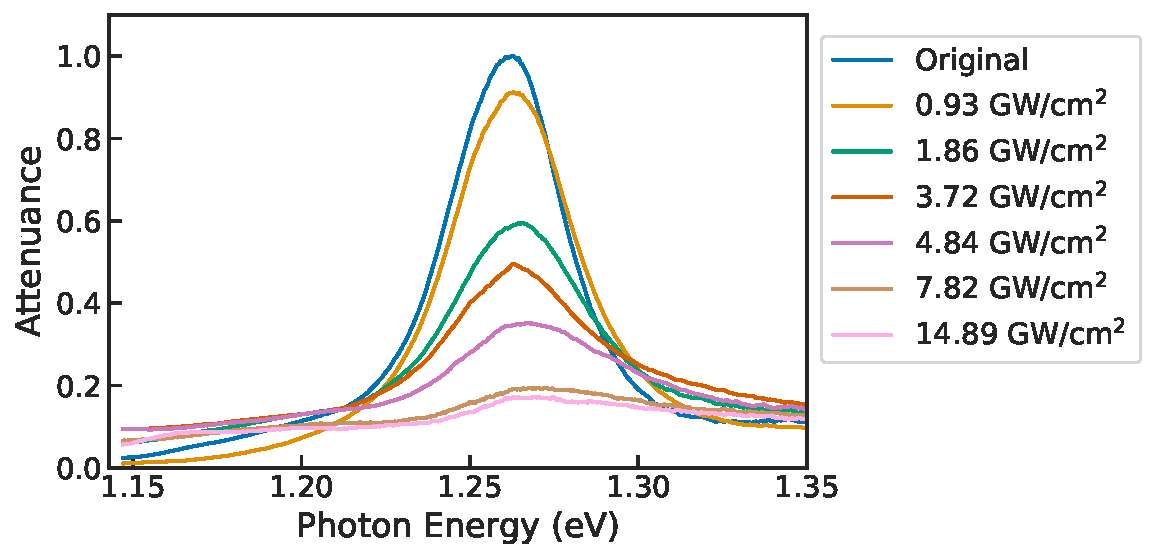
\includegraphics[height=2.4in]{images/chapter_my_data/Weilu_CNT_abs_max_change}
	\caption{Maximum decay of the $E_{11}$ peak observed at the labeled excitation power densities. The top-most trace shows the linear absorption of the spectral region. At higher power densities, the $E_{11}$ resonance diminishes more and more due to the creation of carriers. The peak also slightly blueshifts and broadens.}
	\label{fig:weilu_cnt_max_decay}
\end{figure}

\begin{figure}[H]
	\centering
	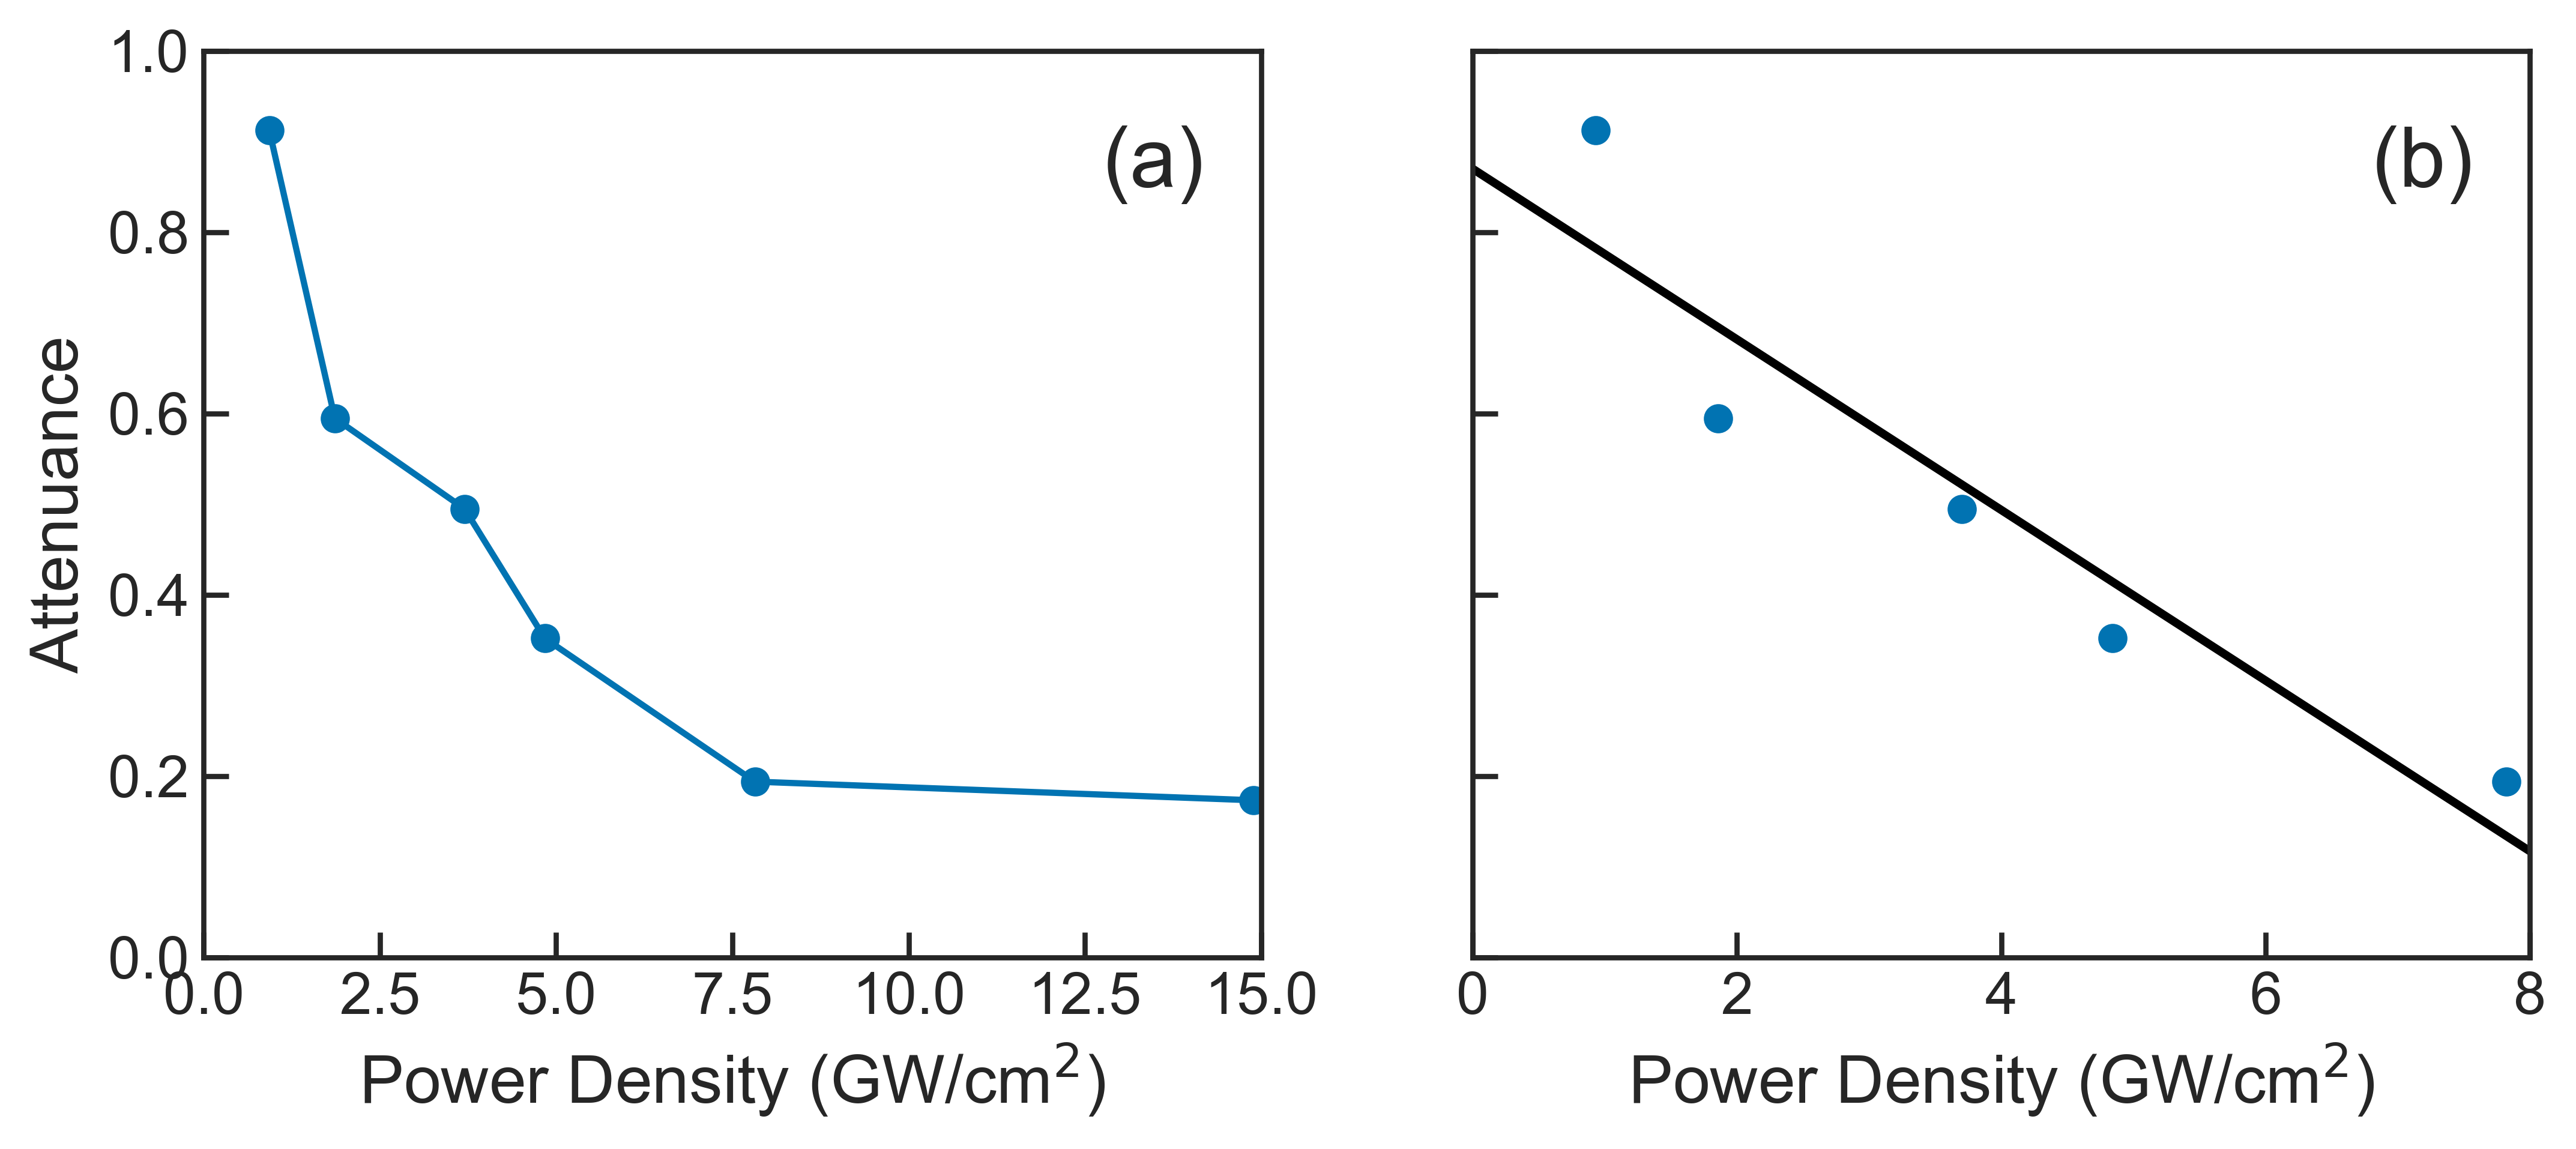
\includegraphics[height=2.4in]{images/chapter_my_data/Weilu_CNT_max_attenuance_and_fit}
	\caption{Maximum attenuance of the $E_{11}$ peak as a function of power density obtained from Figure \ref{fig:weilu_cnt_max_decay}. (a) Photo-bleaching of the $E_{11}$ resonance appears to saturate above a power density of 8 GW/cm$^2$. (b) Below power densities of 8 GW/cm$^2$, the decay of the $E_{11}$ peak is linearly proportional to the power density.}
	\label{fig:weilu_cnt_max_decay_fit}
\end{figure}

\begin{figure}[ht]
	\centering
	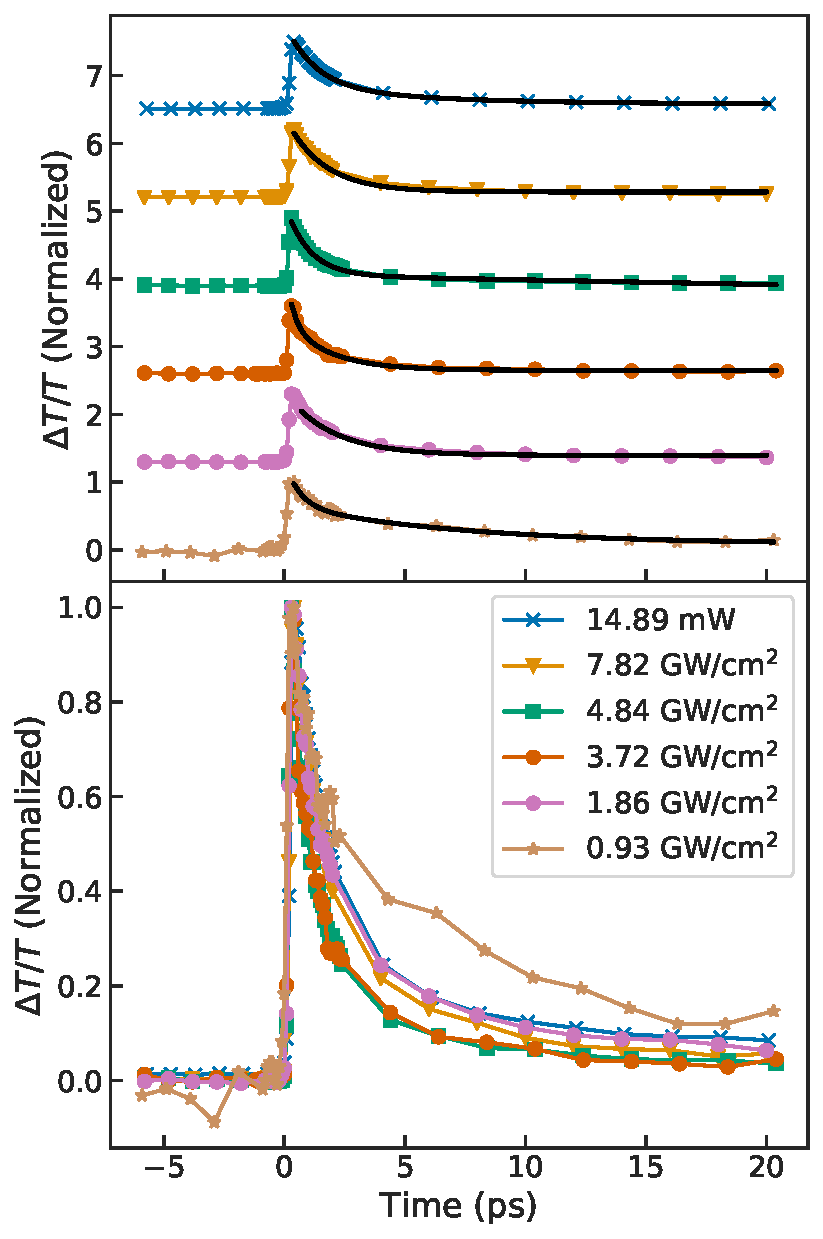
\includegraphics[height=5.4in]{images/chapter_my_data/Weilu_CNT_diff_trans_fits_and_normalized}
	\caption{ Normalized differential transmission measured at the $E_{11}$ resonance at the labeled power densities. (a) Each curve is manually offset for clarity. The solid black lines correspond to fits to the data using a bi-exponential decay model. (b) The differential transmission does not appear to have a significant dependence on the pump power density especially at higher intensities. The dynamics at the lowest intensity are dominated by the slower decay process. At higher intensities, all the measured traces do not show significant deviations from each other as expected from the effects of efficient exciton-exciton annihilation. }
	\label{fig:weilu_cnt_normalized_dt}
\end{figure}




\begin{figure}[ht]
	\centering
	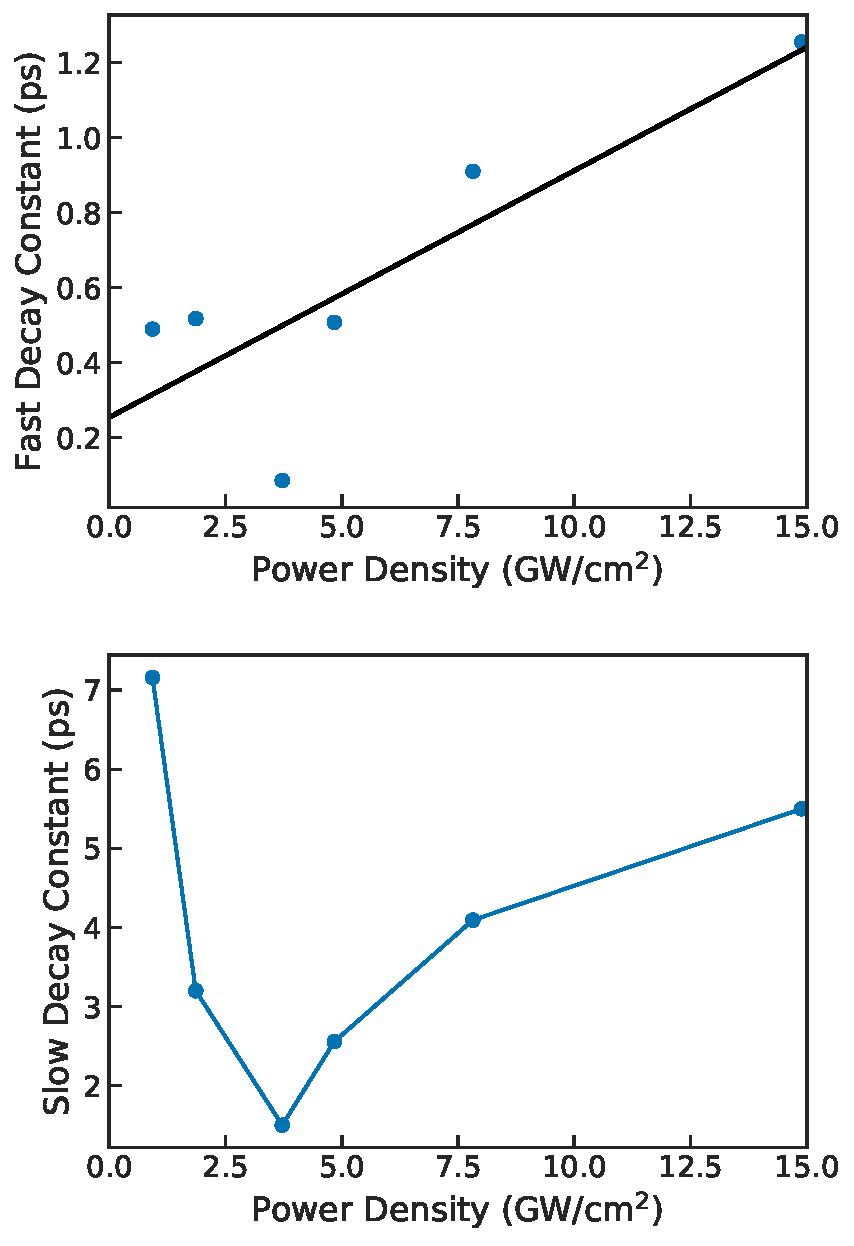
\includegraphics[height=5.4in]{images/chapter_my_data/Weilu_CNT_Fast_Slow_Decay_Const}
	\caption{(a) Fast and (b) slow decay constants extracted from the fits to the data shown in Figure \ref{fig:weilu_cnt_normalized_dt}(a). The the fast decay constant increases linearly with with the power density. This does not corroborate efficient exciton-exciton annihilation, where the fast decay constant would be expected to decrease with the power density rather than increase. The slow decay constant however shows a slightly different trend. While it appears to dominate the dynamics observed at the lower power density it decreases, it diminishes at medium intensities but increases yet again at the highest intensities.}
	\label{fig:weilu_cnt_decay_const}
\end{figure}


\clearpage
\subsection{Polymer-Wrapped (6,5)-Enriched Dispersion}



\begin{figure}[H]%
	\centering
	{\includegraphics[height=2.4in]{images/chapter_my_data/Jan_CNT_ABS_1mW_decay} \phantomsubcaption}
	{\includegraphics[height=2.4in]{images/chapter_my_data/Jan_CNT_ABS_1mW_recovery} \phantomsubcaption}
	\caption{Attenuance traces measured at the indicated time delay after resonantly exciting the $E_{22}$ transition with a power density of 1.9 GW/cm$^2$. (a) Total attenuance showing the decay of the absorption at the $E_{11}$ peak at 1.26 eV as well as the attenuation of the phonon sideband located at 1.35 eV. (b) A close-up of the changes $E_{11}$ spectral region shown in Figure (a). (c) Total attenuance at later times showing the recovery of the $E_{11}$ and phonon sideband peaks. (d) A close-up of the changes $E_{11}$ spectral region shown in Figure (c).}
	\label{fig:jan_cnt_time_traces}
\end{figure}

\begin{figure}[ht]
	\centering
	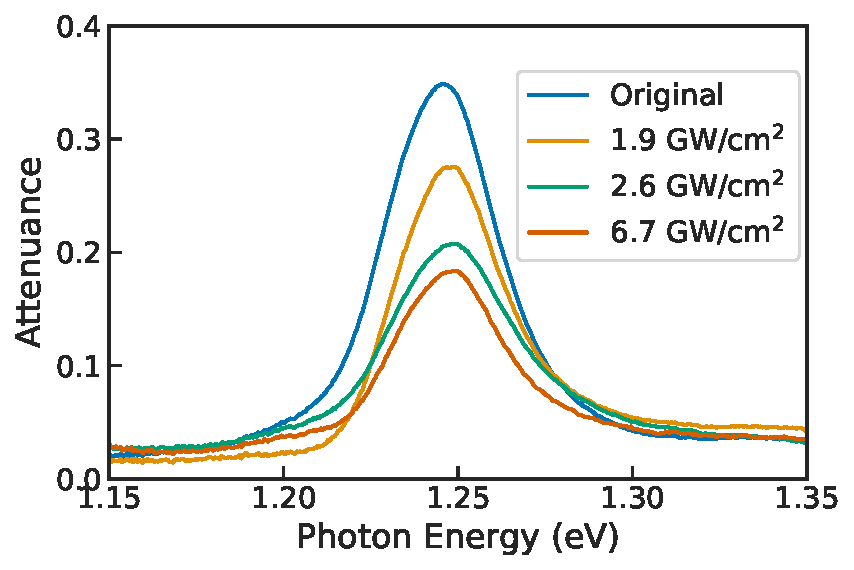
\includegraphics[height=2.4in]{images/chapter_my_data/Jan_CNT_max_abs_change}
	\caption{Maximum decay of the $E_{11}$ peak observed at the labeled excitation power densities. The top-most trace shows the linear absorption of the spectral region. At higher power densities, the $E_{11}$ resonance increasingly diminishes due to the creation of carriers.}
	\label{fig:jan_cnt_max_decay}
\end{figure}

\begin{figure}[H]
	\centering
	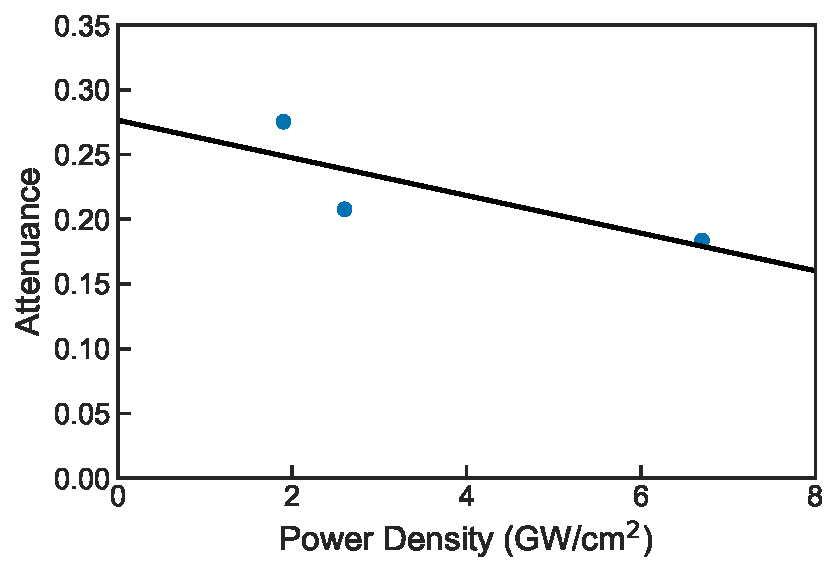
\includegraphics[height=2.4in]{images/chapter_my_data/Jan_CNT_max_attenuance_and_fit}
	\caption{Maximum attenuance of the $E_{11}$ peak as a function of power density obtained from Figure \ref{fig:jan_cnt_max_decay}. The attenuance appears to decrease with the power density in a linear fashion.}
	\label{fig:jan_cnt_max_decay_fit}
\end{figure}

\begin{figure}[ht]
	\centering
	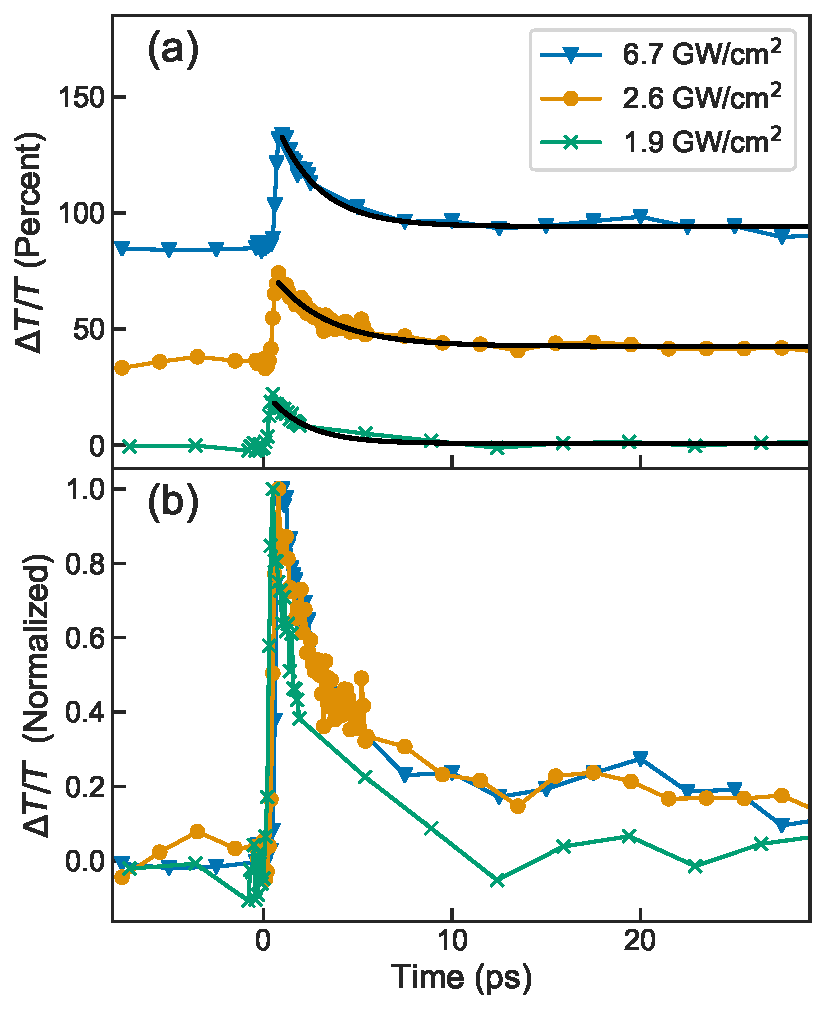
\includegraphics[height=4.4in]{images/chapter_my_data/Jan_CNT_diff_trans_fits_and_normalized}
	\caption{(a) Differential transmission measured at the $E_{11}$ resonance at the labeled power densities. Each curve is manually offset for clarity. The solid black lines correspond to fits to the data using an exponential decay model. (b) Normalized differential transmission measured at the $E_{11}$ transition. The traces do not appear to show a significant dependence on the power density of the optical pump. Furthermore, the signals measured at 2.6 GW/cm$^2$ and 6.7 GW/cm$^2$ overlap each other.}
	\label{fig:jan_cnt_max_normalized_dt}
\end{figure}

\clearpage

\begin{figure}[ht]
	\centering
	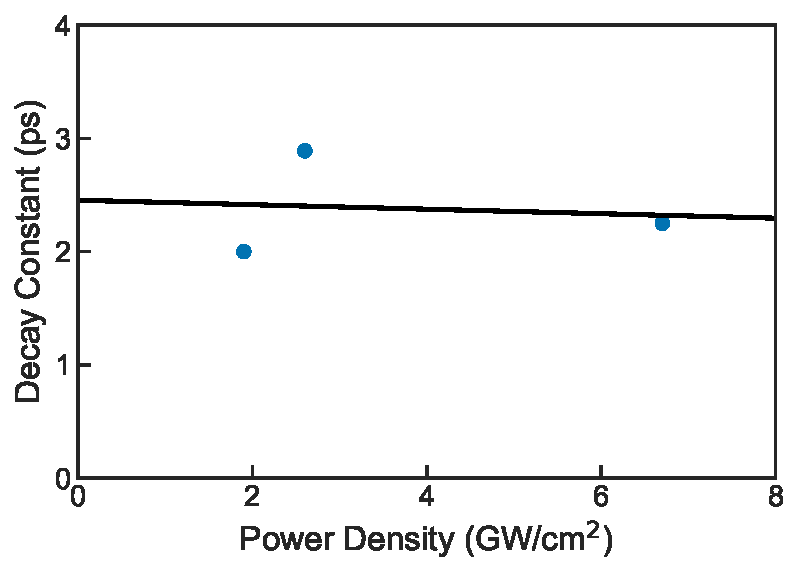
\includegraphics[height=2.5in]{images/chapter_my_data/Jan_CNT_decay_const_fit}
	\caption{Exponential decay constants obtained from Figure \ref{fig:jan_cnt_decay_const}. The decay constants do not show a significant dependence on the power density of the optical pump. }
	\label{fig:jan_cnt_decay_const}
\end{figure}

\section{Discussion}

Figures \ref{fig:weilu_cnt_time_traces} (DOC-Suspended Sample) and \ref{fig:jan_cnt_time_traces} (Polymer-Wrapped Sample) show a very fast response occuring at the $E_{11}$ resonance shortly after resonantly exciting the $E_{22}$ transition. It appears that $E_{22}$ excitons quickly decay to form $E_{11}$ excitons. This observation agrees with work of Manzoni et al (2005) who observed that inter-subband relaxation occurs on a femtosecond timescale.

The two figures also do show some key differences. In Figure \ref{fig:weilu_cnt_time_traces}, the $E_{11}$ peak broadens and blueshifts. This is typically interpreted as an indication of exciton-exciton screening \cite{shah1996ultrafast}. In the presence of a large population of excitons, the Coulomb interactions between electrons and holes become screened. This leads to a reduced binding energy and broadening of $E_{11}$ peak due to the lower stability of excitons. These results differ from the observations by Ostojic et al.\ (2005) as well as Murakami and Kono (2009) who did not observe any change in the positions and linewidths of the optical resonances in their samples.

If exciton-exciton annihilation were indeed efficient, then the significant photo-bleaching of the optical resonances in SWCNTs should not at all be possible as mentioned by Murakami and Kono (2009). Furthermore, the strong attenuation of oscillator strength of the $E_{11}$ peak may suggest that the density of photo-generated excitons exceeds the Mott density of the system. Excitons, being composed of two half-integer spin quasiparticles, are expected to behave as bosons \cite{Ashcroft, laikhtman2007excitons}. Hence, there should not be photo-bleaching of resonance if only excitons are created by the optical pump as bosons are exempt from the Pauli exclusion principle. The results here suggest that Fermions also play a role in the observed carrier dynamics.

Unlike Figure \ref{fig:weilu_cnt_time_traces}, Figure \ref{fig:jan_cnt_time_traces} instead shows a narrowing of the $E_{11}$ resonance, especially on the lower energy region of the $E_{11}$ resonance. This could be a sign of spectral-hole burning. Here, the $E_{11}$ peak is inhomogenously broadened as the dispersion contains an ensemble of (6,5) SWCNTs. As a result the homogenous optical resonances, emerging from individual nanotubes, in the lower energy region of the $E_{11}$ resonance will be the first to become photo-bleached.

Figures \ref{fig:weilu_cnt_max_decay}  (DOC-Suspended Sample) and \ref{fig:jan_cnt_max_decay} (Polymer-Wrapped Sample) show the decay of the $E_{11}$ peak as the power density of the optical pump is increased. In the case of Figure \ref{fig:weilu_cnt_max_decay}, the $E_{11}$ peak almost completely disappears, whereas in Figure \ref{fig:jan_cnt_max_decay}, the limited data does seem to indicate saturation behavior as the change from 2.9 to 6.7 GW/cm$^2$ is almost negligible when compared to the change from 1.9 to 2.6 GW/cm$^2$. The maximum attenuances from these figures are plotted in Figures \ref{fig:weilu_cnt_max_decay_fit} and \ref{fig:jan_cnt_max_decay_fit} respectively. Both figures show that the oscillator strength of the $E_{11}$ peak decreases as the pump intensity increases. Figure \ref{fig:weilu_cnt_max_decay_fit} shows a linear decrease that occurs up until a power density of 7.8 GW/cm$^2$. After that point, the decrease in the attenuance begins to saturate. Due to the limited data collected in Figure \ref{fig:jan_cnt_max_decay_fit} it is more difficult to conclude whether saturation does occur. However, the decrease in the attenuance appears to be somewhat linear as shown by the linear fit to the data.

The changes in differential transmission recorded at the $E_{11}$ resonance do not corroborate the previously reported evidence of efficient exciton-exciton annihilation. Figures \ref{fig:weilu_cnt_normalized_dt} (DOC-Suspended Sample) and \ref{fig:jan_cnt_max_normalized_dt} (Polymer-Wrapped Sample) demonstrate this. In Figure \ref{fig:weilu_cnt_normalized_dt}(a), DOC suspension sample showed carrier dynamics that agree with a bi-exponential fit whereas, those of polymer-wrapped sample shown in Figure \ref{fig:jan_cnt_max_normalized_dt} instead correspond to exponential decays. This suggests that carrier relaxation in the polymer-wrapped sample occurs more slowly. Overall, the normalized differential transmission data measured at the indicated power densities closely overlap one another and a fast initial decay does not dominate the observed dynamics at higher power densities. This result however may not be too surprising as previous transient absorption measurements in the literature also did not observe any nonlinear carrier dynamics associated with efficient exciton-exciton annihilation \cite{ostojic2004interband, manzoni2005intersubband, ma2005femtosecond, luer2009size}.

Furthermore, the scenario presented by dominant exciton-exciton annihilation processes suggests that the initial decay should become faster with increasing power density. The decay constants extracted from the differential transmission data do not exhibit such a trend. Figures \ref{fig:weilu_cnt_decay_const} and \ref{fig:jan_cnt_decay_const} show the extracted decay constants obtained by fitting to the differential transmission measured in each sample respectively. In Figure \ref{fig:weilu_cnt_decay_const}(a), the fast decay constant increases linearly with the power density, whereas in Figure \ref{fig:jan_cnt_decay_const} the decay time does not change significantly.


\section{Conclusions}

In this work, we studied the carrier relaxation dynamics of two ensembles of SWCNTs induced by resonant $E_{22}$ excitation. These two ensembles included SWCNTs disperesed in an aqueous solution using DOC as a surfactant as well as another dispersion of polymer-wrapped SWCNTs dispersed in toluene. In both samples, we observed a fast response at the $E_{11}$ transition after creating $E_{22}$ excitons with the optical pump. In the DOC suspension, the $E_{11}$ peak broadened, blueshifted and was almost completely photo-bleached, suggesting that enough carriers were created to exceed the Mott density. However, in the polymer-wrapped sample, the significant photo-bleaching of the lower energy region of the $E_{11}$ was interpreted as a signature of spectral hole burning.

In addition, the data do not show signs of efficient exciton-exciton annihilation. For the samples studied, the measurements indicate that the dominance of a fast exponential is rather weak and does not appropriately scale with the fluence of the optical pump as expected by time-resolved photoluminenscence measurements. Instead of an intial decay that becomes faster with higher pump intensities, a signature of exciton-exciton annihilation, we observed an intial decay that either slows down with increasing pump intensity or remains roughly constant depending on the sample being studied. In conclusion, the narrative of efficient exciton-exciton may be not be completely conclusive and warrants further study.


\appendix

%\include{append-a}
%\appendix
%\addcontentsline{toc} {chapter}{\numberline {}Appendix A}
%\include{append-a}
%\include{append-b}
%\addcontentsline{toc} {chapter}{\numberline {}Bibliography}{}
%\include{biblio}

%\bibliographystyle{ieeetr}
%\bibliography{PhD_bibliography}
\end{document}
